\documentclass[a4paper,11pt]{article}
\input{/home/tof/Documents/Cozy/latex-include/preambule_doc.tex}
\input{/home/tof/Documents/Cozy/latex-include/preambule_commun.tex}
\newcommand{\showprof}{show them}  % comment this line if you don't want to see todo environment
\setlength{\fboxrule}{0.8pt}
\fancyhead[L]{\fbox{\Large{\textbf{Lang 01}}}}
\fancyhead[C]{\textbf{Minecraft}}
\newdate{madate}{10}{09}{2020}
%\fancyhead[R]{\displaydate{madate}} %\today
\fancyhead[R]{Terminale - NSI}
\fancyfoot[L]{\vspace{1mm}Christophe Viroulaud}
\AtEndDocument{\label{lastpage}}
\fancyfoot[C]{\textbf{Page \thepage/\pageref{lastpage}}}
\fancyfoot[R]{\includegraphics[width=2cm,align=t]{/home/tof/Documents/Cozy/latex-include/cc.png}}
\usepackage{tikz}
\usetikzlibrary{shapes.multipart}
%DODO fin trop compliquée + faire détails instanciation (schéma) + davantage d'exemples basiques
\begin{document}
\begin{center}
    \framebox{Quel paradigme mettre en place pour programmer Minecraft?}
\end{center}
\section{Principes du jeu}
\begin{center}
    \centering
    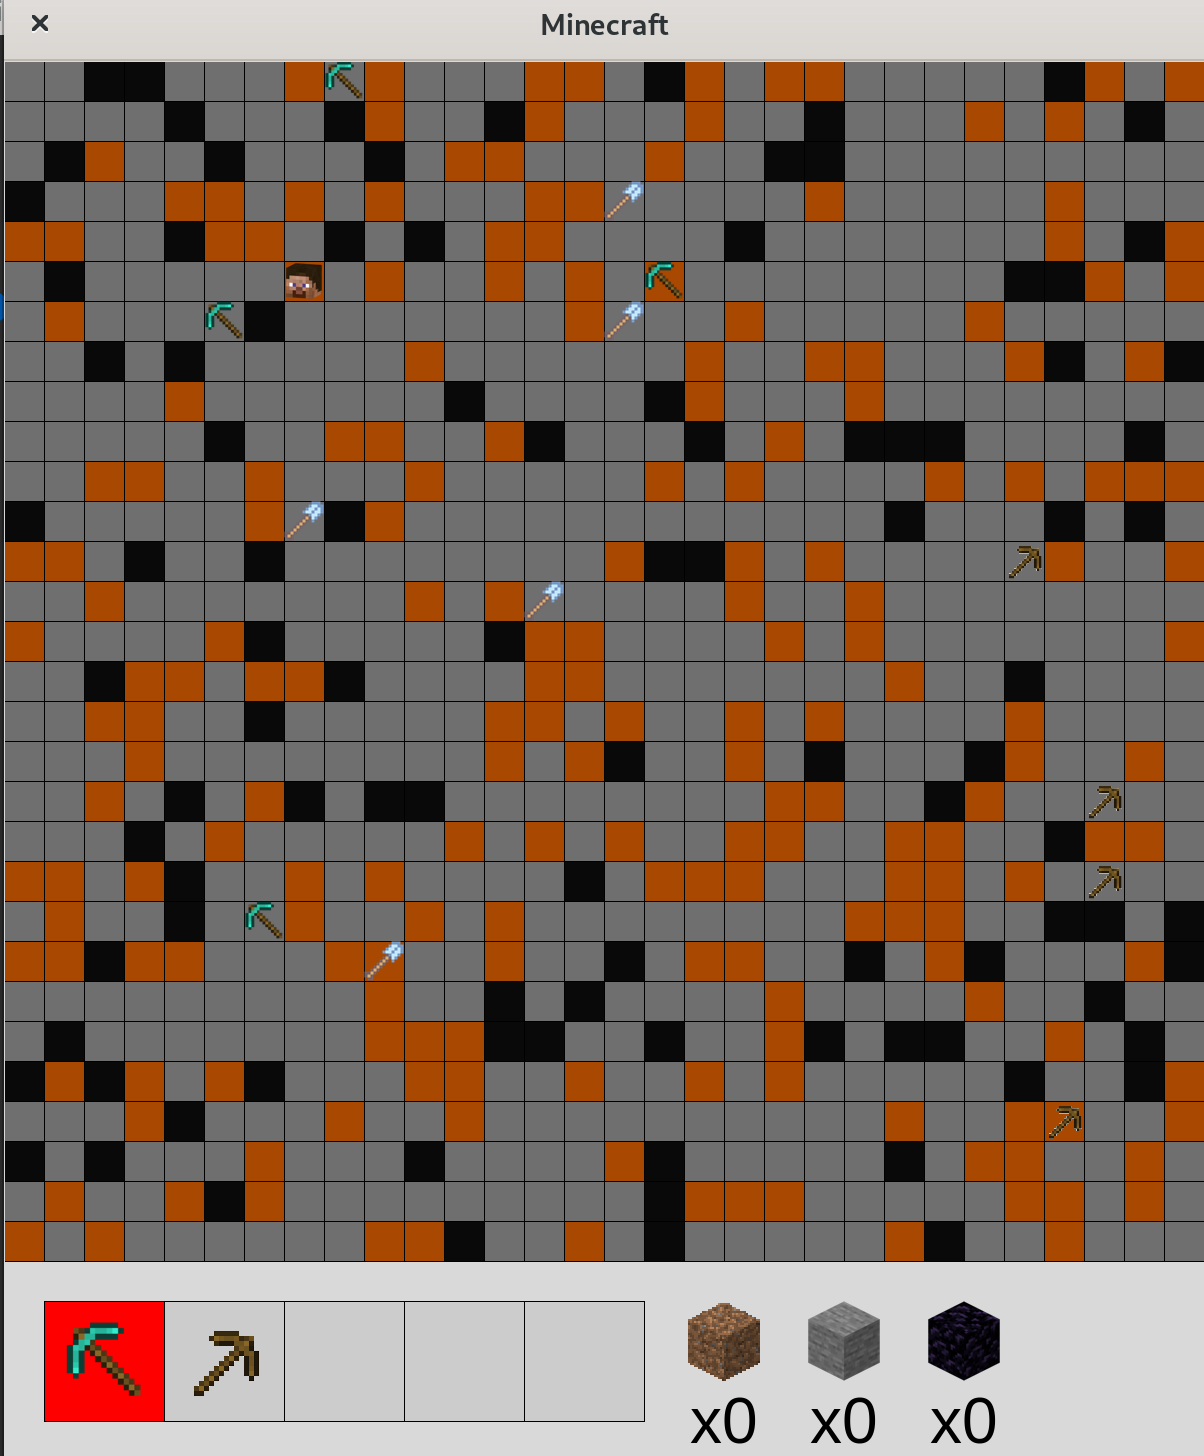
\includegraphics[width=5cm]{ressources/jeu.png}
    \captionof{figure}{Une version simplifiée}
    \label{jeu}
\end{center}
\section{Programmation orienté objet}
\subsection{Définition}
Le \textbf{paradigme objet} consiste à construire des \emph{objets} et les faire interagir entre eux. Un objet représente une entité physique, un concept\dots 
\begin{aretenir}[]
    Un objet possède:
    \begin{itemize}
        \item des caractéristiques: \textbf{les attributs},
        \item des capacités: \textbf{les méthodes}.
    \end{itemize}
\end{aretenir}
\subsection{Modélisation}
\begin{center}
    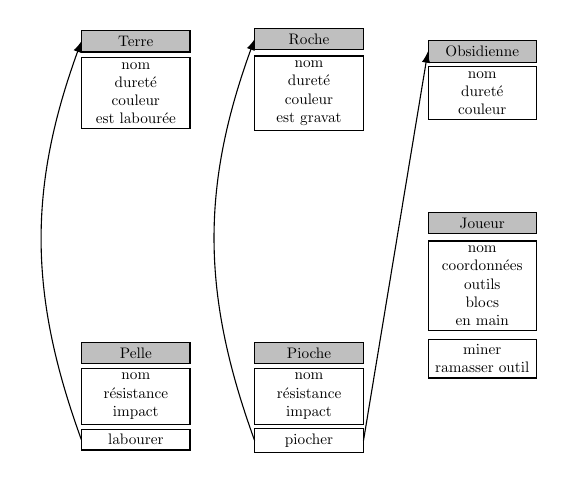
\begin{tikzpicture}[every text node part/.style={align=center},scale=0.55, transform shape]
        \node[draw,fill=gray!50,minimum width=2.5cm, minimum height=0.5cm] (terre) at (0,1.2) {Terre};
        \node[draw,minimum width=2.5cm] at (0,0) {nom \\ dureté \\ couleur \\ est labourée};

        \node[draw,fill=gray!50,minimum width=2.5cm, minimum height=0.5cm] (roche) at (4,1.25) {Roche};
        \node[draw,minimum width=2.5cm] at (4,0) {nom \\ dureté \\ couleur \\ est gravat};

        \node[draw,fill=gray!50,minimum width=2.5cm, minimum height=0.5cm] (obsidienne) at (8,0.96) {Obsidienne};
        \node[draw,minimum width=2.5cm] at (8,0) {nom \\ dureté \\ couleur};


        \node[draw,fill=gray!50,minimum width=2.5cm, minimum height=0.5cm] (pelle) at (0,-6) {Pelle};
        \node[draw,minimum width=2.5cm] at (0,-7) {nom \\ résistance \\ impact};
        \node[draw,minimum width=2.5cm] (labourer) at (0,-8) {labourer};


        \node[draw,fill=gray!50,minimum width=2.5cm, minimum height=0.5cm] (pioche) at (4,-6) {Pioche};
        \node[draw,minimum width=2.5cm] at (4,-7) {nom \\ résistance \\ impact};
        \node[draw,minimum width=2.5cm] (piocher) at (4,-8.02) {piocher};


        \node[draw,fill=gray!50,minimum width=2.5cm, minimum height=0.5cm] (joueur) at (8,-3) {Joueur};
        \node[draw,minimum width=2.5cm] at (8,-4.45) {nom \\ coordonnées \\ outils \\ blocs \\ en main};
        \node[draw,minimum width=2.5cm] at (8,-6.13) {miner \\ ramasser outil};

        \draw[->,>=latex] (labourer.west) to[bend left=20] (terre.west);
        \draw[->,>=latex] (piocher.west) to[bend left=20] (roche.west);
        \draw[->,>=latex] (piocher.east) to (obsidienne.west);

    \end{tikzpicture}
\end{center}
\subsection{Instanciation}
\begin{itemize}
    \item Chaque objet est un modèle qui peut être vu comme un squelette.
    \begin{center}
        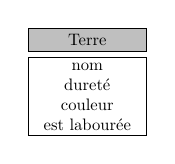
\begin{tikzpicture}[every text node part/.style={align=center},scale=0.6, transform shape]
            \node[draw,fill=gray!50,minimum width=2.5cm, minimum height=0.5cm] (terre) at (0,1.2) {Terre};
            \node[draw,minimum width=2.5cm] at (0,0) {nom \\ dureté\\ couleur\\ est labourée};
        \end{tikzpicture}
    \end{center}
    \item On crée une \textbf{instance} de l'objet. C'est cette instance qui interagit dans le programme.
          \begin{center}
              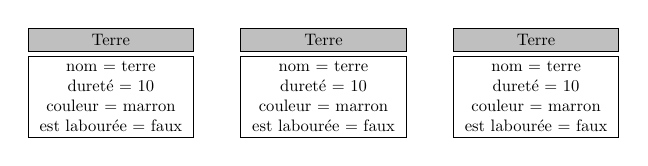
\begin{tikzpicture}[every text node part/.style={align=center},scale=0.6, transform shape]
                  \node[draw,fill=gray!50,minimum width=3.5cm, minimum height=0.5cm] (terre) at (0,1.2) {Terre};
                  \node[draw,minimum width=3.5cm] at (0,0) {nom = terre \\ dureté = 10\\ couleur = marron\\ est labourée = faux};
                  \node[draw,fill=gray!50,minimum width=3.5cm, minimum height=0.5cm] (terre) at (4.5,1.2) {Terre};
                  \node[draw,minimum width=3.5cm] at (4.5,0) {nom = terre \\ dureté = 10\\ couleur = marron\\ est labourée = faux};
                  \node[draw,fill=gray!50,minimum width=3.5cm, minimum height=0.5cm] (terre) at (9,1.2) {Terre};
                  \node[draw,minimum width=3.5cm] at (9,0) {nom = terre \\ dureté = 10\\ couleur = marron\\ est labourée = faux};
              \end{tikzpicture}
          \end{center}
    \item Chaque instance possède ses propres \emph{attributs} et \emph{méthodes}.
\end{itemize}
\section{Implémentation}
\subsection{Créer un objet}
\begin{center}
\begin{lstlisting}[language=Python  , xleftmargin=2em, xrightmargin=2em]
class Terre
\end{lstlisting}
\captionof{code}{Créer une classe}
\label{CODE}
\end{center}
\subsection{Initialiser les attributs}
La \emph{méthode} \texttt{\textbf{\_\_init\_\_}} est appelée automatiquement quand nous instancions un objet.
\begin{center}
\begin{lstlisting}[language=Python , xleftmargin=2em, xrightmargin=2em]
class Pioche:
    def __init__(self, nom: str):
        self.nom = nom
        if nom == "wood_pickaxe":
            self.resistance = 30
            self.impact = 5
        elif nom == "diamond_pickaxe":
            self.resistance = 100
            self.impact = 100
\end{lstlisting}
\captionof{code}{Les attributs sont initialisés dans le \emph{constructeur}.}
\label{CODE}
\end{center}

\subsection{Définir les méthodes}
\begin{aretenir}
    On appelle \textbf{méthode} une fonction interne à la classe de l'objet. 

    En Python, le premier paramètre est \textbf{toujours} \textbf{\texttt{self}}. C'est un attribut \textbf{interne} à la classe.
\end{aretenir}
\begin{center}
    \begin{lstlisting}[language=Python, xleftmargin=2em, xrightmargin=2em]
def piocher(self, bloc: object) -> bool:
    bloc.durete -= self.impact
    self.resistance -= USURE
    if self.resistance <= 0:
        return False
    return True
\end{lstlisting}
    \end{center}
\end{document}
